%=====================================================================
\section{The experiments: how to read them}
\label{sec:expintro}

Each experiment changes \emph{one} number in the model (Table~\ref{tab:design}) by a comparable amount, re-solves
all 560 instances, and measures the change against the baseline on the instances feasible in both. E1--E8 are run
by both methods; E9--E10 (Sections~\ref{sec:e9}--\ref{sec:e10}) by the retrained RL policy. Every variant is
presented as \emph{theory} (a proposition read off the model), \emph{result} (the measured table), \emph{practical
cause}, and \emph{support}.

\begin{table}[H]
\centering\small
\caption{The seven experiments and the part of the model each one moves.}
\label{tab:design}
\begin{adjustbox}{max width=\linewidth}
\begin{tabular}{@{}llll@{}}
\toprule
exp. & factor changed & where it enters & variants (baseline) \\
\midrule
E1 & van tariff $p^{\mathrm M}$ & $Z_5$ and the premium $\Pi_i$ \eqref{eq:delP} & 15, 35 Rs/kWh (25) \\
E2 & mobile chargers: vans, seats & fleet $|M|$, seats $Q_m$ in \eqref{eq:vancap} & 3/7 vans, 4/8 seats (5, 6) \\
E5 & value of charging time & $c^{\mathrm C,\mathrm P}$, $\omega$ in $Z_6$ & $\pm25$\,\% \\
E6 & money sensitivity $\mu^{0}$ & $\mu_i$ in $Z_1,Z_5$ (per segment) & $\pm25$\,\% \\
E8 & van battery $B_m$ & battery \eqref{eq:vanbatt} & 200 kWh (150) \\
E9 & station capacity & guns $|G_f|$, power $P^{\mathrm F}$ in \eqref{eq:gunload},\eqref{eq:tau} & 1/4 guns, 11/44 kW (2, 22) \\
E10 & charging demand & energy $E_i$ (everywhere) & $\times0.75,\times1.25$ (1) \\
\bottomrule
\end{tabular}
\end{adjustbox}
\end{table}

\begin{figure}[H]
\centering
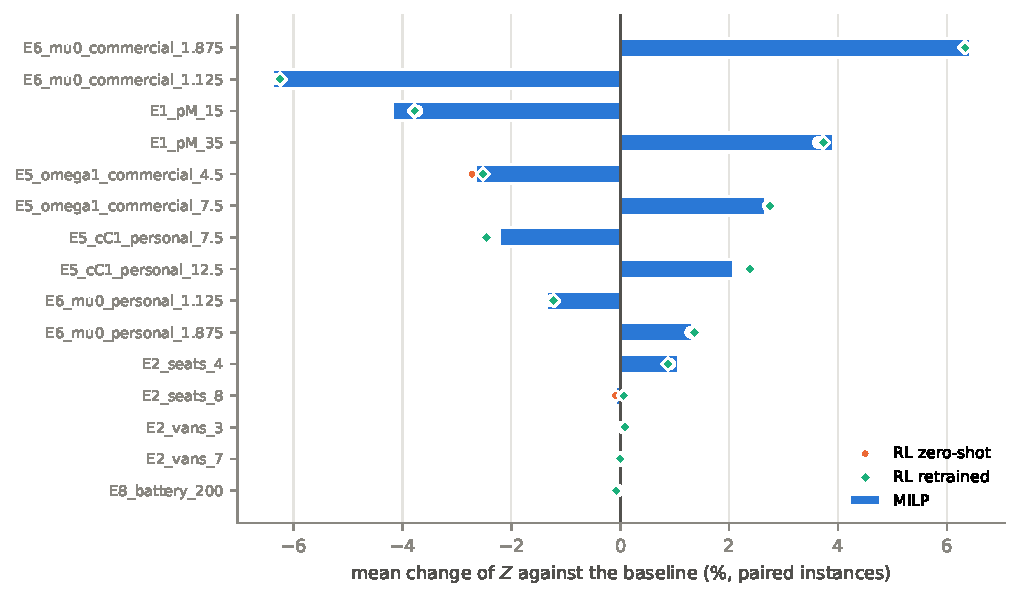
\includegraphics[width=0.9\textwidth]{figures/exp_tornado.pdf}
\caption{Overview: mean change of $Z$ for every E1--E8 variant (bars: MILP; markers: RL zero-shot and retrained),
sorted by size. The two methods land on top of each other.}
\label{fig:tornado}
\end{figure}

%---------------------------------------------------------------------
\subsection{E5 --- the value of charging time}
\label{sec:e5}
E5 raises and lowers, by $\pm25$\,\%, the richest private owner's value of a station minute
($c^{\mathrm C,\mathrm P}$) and the top commercial downtime rate ($\omega^{1}$).

\begin{proposition}[station-time value lifts cost \emph{and} van use for personal cars; downtime rate lifts only cost]
\label{prop:e5}
(a) $\partial Z/\partial c^{\mathrm C,\mathrm P}=\sum_{i\in\mathrm P}\tau^{\mathrm F}_iy_i\cdot\partial c^{\mathrm C,\mathrm P}/\partial(\cdot)\ge0$,
and $\partial\Delta^{\mathrm P}_i/\partial c^{\mathrm C,\mathrm P}=-\tau^{\mathrm F}_i<0$, so a higher personal
value of station time raises $Z$ and makes the van relatively better for personal cars.
(b) Scaling $\omega$ (with $c^{\mathrm D,\mathrm C}=c^{\mathrm C,\mathrm C}=c^{\mathrm V,\mathrm C}=\omega$) multiplies
every commercial time cost, and in $\Delta^{\mathrm C}_i=\mu^{\mathrm C}\Pi_i+\kappa_i-\omega D_i-\delta q^{\mathrm F}_i$
scales only the $\omega D_i$ term, so it changes the cost \emph{level} but barely the commercial assignment.
\end{proposition}
\begin{proof}
(a) $c^{\mathrm C,\mathrm P}$ multiplies $\tau^{\mathrm F}_iy_i$ in $Z_6$ for personal FCS users, a non-negative
quantity, giving the stated sign; it enters $\Delta^{\mathrm P}_i$ \eqref{eq:delP} only through $-c^{\mathrm C,\mathrm P}\tau^{\mathrm F}_i$,
so $\partial\Delta^{\mathrm P}_i/\partial c^{\mathrm C,\mathrm P}=-\tau^{\mathrm F}_i<0$: $\Delta^{\mathrm P}_i$
falls, crossing zero for more cars, so more personal cars take vans. (b) For commercial cars $Z_{6,i}=\omega(C_i-r_i)+\delta q^{\mathrm F}_i$
is linear in $\omega$, so $\partial Z/\partial\omega>0$; in $\Delta^{\mathrm C}_i$ the station and van options are
both priced at $\omega$, so the $\theta$-threshold $\theta^{*}_{i,\mathrm C}$ moves only through the ratio, not the
level --- the choice is first-order invariant.
\end{proof}

\textbf{Result.}
\begin{table}[H]\centering
\caption{E5. Rows: MILP, RL zero-shot, RL retrained. $\Delta$ in \% against the baseline (paired instances).}
\scriptsize
\begin{adjustbox}{max width=\linewidth}
\begin{tabular}{@{}lrrrrrrrrrrr@{}}
\toprule
method & valid & paired & new & lost & \shortstack{$\Delta Z$\\\%} & \shortstack{$\Delta$\\oper. \%} & \shortstack{$\Delta$\\cust. \%} & \shortstack{van \%\\personal} & van \% comm. & vans used & \shortstack{gap to\\MILP \%} \\
\midrule
\multicolumn{12}{@{}l}{\textbf{E5\_cC1\_personal\_7.5}: personal $c^{C,1}$ = 7.5 ($-$25 \%)} \\
MILP & 473 & 472 & 1 & 2 & $-$2.21 & $-$1.15 & $-$2.59 & 19.9 $\to$ 14.1 & 0.7 $\to$ 0.8 & 2.13 & -- \\
RL zero-shot & 499 & 499 & 0 & 1 & $-$2.49 & $-$0.21 & $-$3.45 & 6.7 $\to$ 5.5 & 0.9 $\to$ 0.9 & 2.20 & 0.56 \\
RL retrained & 500 & 499 & 1 & 1 & $-$2.46 & $-$0.59 & $-$3.24 & 6.7 $\to$ 3.9 & 0.9 $\to$ 0.8 & 2.19 & 0.56 \\
\multicolumn{12}{@{}l}{\textbf{E5\_cC1\_personal\_12.5}: personal $c^{C,1}$ = 12.5 ($+$25 \%)} \\
MILP & 473 & 472 & 1 & 2 & $+$2.08 & $+$2.75 & $+$1.84 & 19.9 $\to$ 29.4 & 0.7 $\to$ 0.7 & 2.37 & -- \\
RL zero-shot & 502 & 500 & 2 & 0 & $+$2.45 & $+$0.32 & $+$3.37 & 6.7 $\to$ 8.0 & 0.9 $\to$ 0.8 & 2.23 & 1.22 \\
RL retrained & 500 & 500 & 0 & 0 & $+$2.38 & $+$0.93 & $+$3.02 & 6.7 $\to$ 11.7 & 0.9 $\to$ 0.6 & 2.26 & 1.14 \\
\multicolumn{12}{@{}l}{\textbf{E5\_omega1\_commercial\_4.5}: commercial downtime rate at $\theta=1$: 4.5 ($-$25 \%)} \\
MILP & 472 & 471 & 1 & 3 & $-$2.67 & $-$0.17 & $-$3.80 & 19.9 $\to$ 19.6 & 0.7 $\to$ 0.7 & 2.17 & -- \\
RL zero-shot & 500 & 499 & 1 & 1 & $-$2.72 & $-$0.13 & $-$3.86 & 6.7 $\to$ 6.5 & 0.9 $\to$ 0.8 & 2.19 & 0.82 \\
RL retrained & 500 & 499 & 1 & 1 & $-$2.52 & $+$0.17 & $-$3.69 & 6.7 $\to$ 7.6 & 0.9 $\to$ 0.6 & 2.23 & 0.98 \\
\multicolumn{12}{@{}l}{\textbf{E5\_omega1\_commercial\_7.5}: commercial downtime rate at $\theta=1$: 7.5 ($+$25 \%)} \\
MILP & 475 & 472 & 3 & 2 & $+$2.66 & $+$0.26 & $+$3.81 & 19.9 $\to$ 19.6 & 0.7 $\to$ 0.7 & 2.20 & -- \\
RL zero-shot & 500 & 500 & 0 & 0 & $+$2.72 & $+$0.26 & $+$3.82 & 6.7 $\to$ 6.9 & 0.9 $\to$ 0.9 & 2.24 & 0.83 \\
RL retrained & 499 & 499 & 0 & 1 & $+$2.75 & $+$0.14 & $+$3.92 & 6.7 $\to$ 7.0 & 0.9 $\to$ 0.8 & 2.22 & 0.86 \\
\bottomrule
\end{tabular}
\end{adjustbox}

\end{table}
Personal $c^{\mathrm C,\mathrm P}$ moves $Z$ by about $-2.2$ / $+2.1$\,\% \emph{and} swings the personal van share
(19.9\,\% $\to$ 14.1\,\% when station time is valued less, $\to$ 29.4\,\% when valued more). Commercial $\omega^{1}$
moves $Z$ by about $\pm2.7$\,\% but leaves the van shares unchanged (personal $\approx$19.6\,\%, commercial 0.7\,\%).

\practical{When rich private owners hate station time more, the operator buys them out of the queue with vans ---
so the personal van share rises and the operator's cost goes up with it. A taxi's drive, charge and van minutes
all cost the \emph{same} downtime rate, so raising $\omega$ makes the station \emph{and} the van dearer in lockstep:
the taxi's bill grows but its best option does not change.}

\support{Both methods (MILP and the two RL rows) agree on sign and size. The split outcome --- $c^{\mathrm C,\mathrm P}$
changes the \emph{assignment}, $\omega$ only the \emph{level} --- is exactly Proposition~\ref{prop:e5}, and the van-share
move for $c^{\mathrm C,\mathrm P}$ is visible band-by-band in Figure~\ref{fig:expincome}.}

%---------------------------------------------------------------------
\subsection{E6 --- money sensitivity}
\label{sec:e6}
E6 changes, by $\pm25$\,\%, the poorest customer's money sensitivity $\mu^{0}$, per segment.

\begin{proposition}[the commercial money sensitivity is the strongest cost lever]
\label{prop:e6}
$\mu_i$ multiplies the felt driving $Z_1$ and the felt tariff $Z_5$, so $\partial Z/\partial\mu^{s,0}
=\sum_{i\in s}\big(c^{\mathrm{EV}}\!\sum_f d_{if}Y_{if}+E_i(p^{\mathrm F}y_i+p^{\mathrm M}z_i)\big)\cdot\partial\mu_i/\partial\mu^{s,0}\ge0$.
This is largest for $s=\mathrm C$ because commercial cars are the majority and, being low-income, have $\mu_i$ near
$\mu^{\mathrm C,0}$; and it is small for $s=\mathrm P$ because rich personal cars have $\mu_i$ near the \emph{fixed}
$\mu^{\mathrm P,1}$. The assignment is nearly invariant: $\mu$ scales the station and van tariff together, moving
only the premium term $\mu\Pi_i$ in $\Delta_i$.
\end{proposition}
\begin{proof}
$Z_5=\sum_i\mu_iE_i(p^{\mathrm F}y_i+p^{\mathrm M}z_i)$ and $Z_1$ are linear in each $\mu_i$; by \eqref{eq:lines}
$\partial\mu_i/\partial\mu^{s,0}=(1-\theta_i)\mathbf 1[s_i=s]\ge0$, which is near $1$ for low-income cars and near
$0$ for high-income ones, giving the stated magnitudes. In $\Delta_i$, $\mu$ appears only in $\mu_i\Pi_i$; since
both the FCS and van tariffs scale with $\mu_i$, only the \emph{difference} $\Pi_i=(p^{\mathrm M}-p^{\mathrm F})E_i-c^{\mathrm{EV}}d_{if}$
is re-weighted, a small part of $\Delta_i$, so the chosen resource rarely flips.
\end{proof}

\textbf{Result.}
\begin{table}[H]\centering
\caption{E6. Commercial $\mu^{0}$ is the single largest lever; personal $\mu^{0}$ is minor.}
\scriptsize
\begin{adjustbox}{max width=\linewidth}
\begin{tabular}{@{}lrrrrrrrrrrr@{}}
\toprule
method & valid & paired & new & lost & \shortstack{$\Delta Z$\\\%} & \shortstack{$\Delta$\\oper. \%} & \shortstack{$\Delta$\\cust. \%} & \shortstack{van \%\\personal} & van \% comm. & vans used & \shortstack{gap to\\MILP \%} \\
\midrule
\multicolumn{12}{@{}l}{\textbf{E6\_mu0\_personal\_1.125}: personal $\mu^0$ = 1.125 ($-$25 \%)} \\
MILP & 473 & 472 & 1 & 2 & $-$1.35 & $-$0.01 & $-$1.96 & 19.9 $\to$ 19.8 & 0.7 $\to$ 0.6 & 2.18 & -- \\
RL zero-shot & 500 & 499 & 1 & 1 & $-$1.28 & $+$0.10 & $-$1.89 & 6.7 $\to$ 7.0 & 0.9 $\to$ 0.9 & 2.21 & 0.92 \\
RL retrained & 501 & 500 & 1 & 0 & $-$1.22 & $+$0.07 & $-$1.79 & 6.7 $\to$ 7.8 & 0.9 $\to$ 0.7 & 2.21 & 0.95 \\
\multicolumn{12}{@{}l}{\textbf{E6\_mu0\_personal\_1.875}: personal $\mu^0$ = 1.875 ($+$25 \%)} \\
MILP & 475 & 473 & 2 & 1 & $+$1.33 & $-$0.15 & $+$2.04 & 19.9 $\to$ 18.9 & 0.7 $\to$ 0.7 & 2.18 & -- \\
RL zero-shot & 500 & 499 & 1 & 1 & $+$1.29 & $-$0.03 & $+$1.89 & 6.7 $\to$ 6.5 & 0.9 $\to$ 0.8 & 2.21 & 0.80 \\
RL retrained & 499 & 499 & 0 & 1 & $+$1.36 & $+$0.10 & $+$1.94 & 6.7 $\to$ 7.3 & 0.9 $\to$ 0.8 & 2.22 & 0.84 \\
\multicolumn{12}{@{}l}{\textbf{E6\_mu0\_commercial\_1.125}: commercial $\mu^0$ = 1.125 ($-$25 \%)} \\
MILP & 475 & 474 & 1 & 0 & $-$6.38 & $+$0.05 & $-$9.40 & 19.9 $\to$ 19.6 & 0.7 $\to$ 0.7 & 2.20 & -- \\
RL zero-shot & 499 & 499 & 0 & 1 & $-$6.31 & $+$0.07 & $-$9.18 & 6.7 $\to$ 6.8 & 0.9 $\to$ 0.9 & 2.21 & 0.87 \\
RL retrained & 500 & 500 & 0 & 0 & $-$6.25 & $-$0.12 & $-$9.01 & 6.7 $\to$ 7.1 & 0.9 $\to$ 0.8 & 2.19 & 0.91 \\
\multicolumn{12}{@{}l}{\textbf{E6\_mu0\_commercial\_1.875}: commercial $\mu^0$ = 1.875 ($+$25 \%)} \\
MILP & 475 & 473 & 2 & 1 & $+$6.43 & $+$0.06 & $+$9.47 & 19.9 $\to$ 19.8 & 0.7 $\to$ 0.7 & 2.19 & -- \\
RL zero-shot & 500 & 499 & 1 & 1 & $+$6.34 & $+$0.04 & $+$9.19 & 6.7 $\to$ 6.8 & 0.9 $\to$ 0.9 & 2.21 & 0.80 \\
RL retrained & 500 & 499 & 1 & 1 & $+$6.33 & $+$0.12 & $+$9.15 & 6.7 $\to$ 7.8 & 0.9 $\to$ 0.6 & 2.21 & 0.79 \\
\bottomrule
\end{tabular}
\end{adjustbox}

\end{table}
Commercial $\mu^{0}$ moves $Z$ by $\mp6.4$\,\%, almost all on the customers' side ($\mp9.4$\,\%); personal $\mu^{0}$
moves it only $\pm1.3$\,\%. Van shares stay at about 19--20\,\% (personal) and 0.6--0.7\,\% (commercial) throughout.

\practical{Seven in ten customers are commercial and most are poor, so their money sensitivity multiplies the
biggest slice of the bill --- the tariff ($Z_5$, \fshareZFive\,\% of $Z$). Nudging how a poor taxi driver feels a
rupee therefore swings the whole cost. But it makes the station and the van dearer in the same proportion, so
nobody switches resource.}

\support{The $\pm6.4$\,\% is reproduced by MILP and both RL rows. Its size is predicted by the cost anatomy
(Section~\ref{sec:basemilp}: the tariff is \fshareZFive\,\% of $Z$ and most of it is commercial), and its
near-zero effect on the assignment is Proposition~\ref{prop:e6}.}

%---------------------------------------------------------------------
\subsection{E1 --- the van tariff}
\label{sec:e1}
E1 sets the van tariff $p^{\mathrm M}$ to 15 (no premium over the FCS) and 35 Rs/kWh (baseline 25).

\begin{proposition}[the van tariff is the lever on \emph{who} gets a van]
\label{prop:e1}
A higher $p^{\mathrm M}$ cannot lower the optimal cost, and shrinks the set of EVs assigned to vans:
$\partial Z^{*}/\partial p^{\mathrm M}\ge0$ and $\partial\Delta_i/\partial p^{\mathrm M}=\mu_iE_i>0$, so the
van-choice region $\{\Delta_i<0\}$ contracts as $p^{\mathrm M}$ rises.
\end{proposition}
\begin{proof}
$p^{\mathrm M}$ enters $Z$ only through $Z_5=\sum_i\mu_iE_ip^{\mathrm M}z_i$ with coefficient $\mu_iE_iz_i\ge0$, so
raising it weakly raises the cost of \emph{every} feasible plan and hence the optimum (an envelope/monotonicity
argument: the feasible set is unchanged and the objective rises pointwise). In the margin \eqref{eq:delP}--\eqref{eq:delC},
$p^{\mathrm M}$ appears through $\Pi_i=(p^{\mathrm M}-p^{\mathrm F})E_i-c^{\mathrm{EV}}d_{if}$, so
$\partial\Delta_i/\partial p^{\mathrm M}=\mu_iE_i>0$: each $\Delta_i$ rises, so fewer EVs satisfy $\Delta_i<0$.
\end{proof}

\textbf{Result.}
\begin{table}[H]\centering
\caption{E1. Van tariff $p^{\mathrm M}=15$ (no premium) and 35 Rs/kWh.}
\scriptsize
\begin{adjustbox}{max width=\linewidth}
\begin{tabular}{@{}lrrrrrrrrrrr@{}}
\toprule
method & valid & paired & new & lost & \shortstack{$\Delta Z$\\\%} & \shortstack{$\Delta$\\oper. \%} & \shortstack{$\Delta$\\cust. \%} & \shortstack{van \%\\personal} & van \% comm. & vans used & \shortstack{gap to\\MILP \%} \\
\midrule
\multicolumn{12}{@{}l}{\textbf{E1\_pM\_15}: $p^M$ = 15 Rs/kWh (= $p^F$)} \\
MILP & 471 & 470 & 1 & 4 & $-$4.19 & $+$3.69 & $-$7.80 & 19.8 $\to$ 31.4 & 0.7 $\to$ 1.4 & 2.40 & -- \\
RL zero-shot & 500 & 499 & 1 & 1 & $-$3.74 & $+$0.45 & $-$5.66 & 6.7 $\to$ 8.4 & 0.9 $\to$ 1.0 & 2.22 & 1.31 \\
RL retrained & 499 & 499 & 0 & 1 & $-$3.78 & $+$1.04 & $-$5.97 & 6.7 $\to$ 11.3 & 0.9 $\to$ 1.0 & 2.26 & 1.25 \\
\multicolumn{12}{@{}l}{\textbf{E1\_pM\_35}: $p^M$ = 35 Rs/kWh} \\
MILP & 477 & 474 & 3 & 0 & $+$3.91 & $-$1.39 & $+$6.53 & 19.9 $\to$ 13.5 & 0.7 $\to$ 0.8 & 2.12 & -- \\
RL zero-shot & 499 & 498 & 1 & 2 & $+$3.64 & $-$0.36 & $+$5.49 & 6.7 $\to$ 5.1 & 0.9 $\to$ 0.8 & 2.18 & 0.58 \\
RL retrained & 500 & 499 & 1 & 1 & $+$3.73 & $-$0.76 & $+$5.80 & 6.7 $\to$ 1.1 & 0.9 $\to$ 0.9 & 2.18 & 0.64 \\
\bottomrule
\end{tabular}
\end{adjustbox}

\end{table}
\begin{figure}[H]\centering
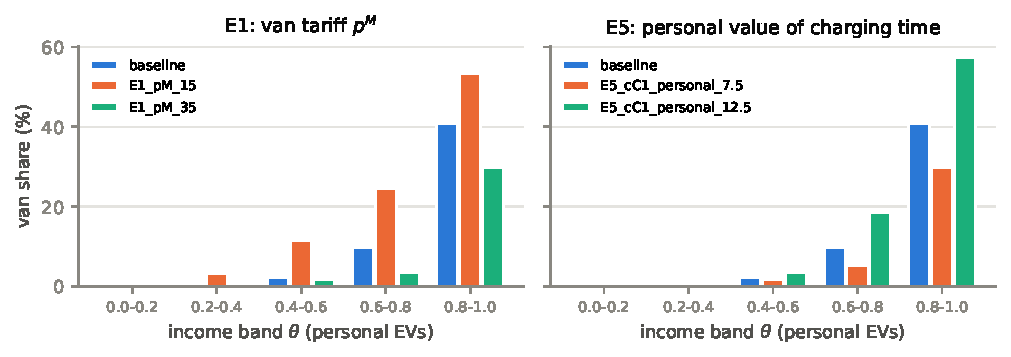
\includegraphics[width=0.95\textwidth]{figures/exp_income.pdf}
\caption{Personal van share by income band: E1 (van tariff) and E5 (personal value of charging time).}
\label{fig:expincome}
\end{figure}
No premium ($p^{\mathrm M}=15$): $Z$ falls about 4.2\,\% --- customers save 7.8\,\%, the operator pays 3.7\,\% more
(more vans dispatched and dearer van energy) --- and the personal van share rises 19.8\,\% $\to$ 31.4\,\%, spreading
down the income scale (Figure~\ref{fig:expincome}). A doubled premium ($35$): $Z$ rises 3.9\,\% and the personal
van share falls to 13.5\,\%.

\practical{The premium is the price of the ``driver-free'' convenience. Cheaper vans let the operator extend that
convenience further down the income scale --- but by rule \textbf{(T1)} the buyers are mostly rich private owners,
so making vans cheaper mostly subsidises them while the operator's own bill goes up.}

\support{Proposition~\ref{prop:e1} forces $\partial Z^{*}/\partial p^{\mathrm M}\ge0$; the direction check
(Section~\ref{sec:validation}) confirms it on the proven optima with zero violations, and the band-by-band shift
of Figure~\ref{fig:expincome} matches the threshold rule \textbf{(T3)}. MILP and RL agree on the cost move and the
direction of the van-share move.}

%---------------------------------------------------------------------
\subsection{E2 --- mobile chargers (fleet size and seats)}
\label{sec:e2}
E2 is the first of the three ``analysis'' factors: the \textbf{number of mobile chargers}. It sets the fleet to 3
or 7 vans (baseline 5) and the seats per van to 4 or 8 (baseline 6).

\begin{proposition}[fleet size buys feasibility, not cost; seats buy cost]
\label{prop:e2}
Enlarging $|M|$ or $Q_m$ only \emph{relaxes} the capacity constraint \eqref{eq:vancap}, so the optimal cost is
non-increasing in both and the feasible set grows. If the fleet is not binding at the optimum, the optimum is
unchanged (only feasibility can change); cutting $Q_m$ tightens \eqref{eq:vancap} and forces more vans to be
dispatched, raising $Z_3$ (and $Z_2$).
\end{proposition}
\begin{proof}
$|M|$ and $Q_m$ appear only on the right-hand side of \eqref{eq:vancap} (and $|M|$ in the routing constraints),
which bound the assignment; increasing them enlarges the feasible region, so $\min Z$ is non-increasing (a larger
feasible set cannot have a higher minimum). By complementary slackness, if \eqref{eq:vancap} is slack at the
optimum a small change of its right-hand side leaves the optimal solution --- and $Z$ --- unchanged; the only
possible change is that a previously infeasible instance becomes feasible. Cutting $Q_m$ removes feasible plans;
serving the same EVs then needs more dispatched vans $u_m$, each adding $c^{\mathrm F}_m$ to $Z_3$.
\end{proof}

\textbf{Result.}
\begin{table}[H]\centering
\caption{E2. 3/7 vans and 4/8 seats. ``new''/``lost'': instances gained/lost against the baseline.}
\scriptsize
\begin{adjustbox}{max width=\linewidth}
\begin{tabular}{@{}lrrrrrrrrrrr@{}}
\toprule
method & valid & paired & new & lost & \shortstack{$\Delta Z$\\\%} & \shortstack{$\Delta$\\oper. \%} & \shortstack{$\Delta$\\cust. \%} & \shortstack{van \%\\personal} & van \% comm. & vans used & \shortstack{gap to\\MILP \%} \\
\midrule
\multicolumn{12}{@{}l}{\textbf{E2\_vans\_3}: 3 vans} \\
MILP & 441 & 441 & 0 & 33 & $-$0.04 & $-$0.53 & $+$0.20 & 19.4 $\to$ 17.4 & 0.2 $\to$ 0.1 & 1.96 & -- \\
RL zero-shot & 465 & 465 & 0 & 35 & $+$0.02 & $-$0.27 & $+$0.15 & 6.4 $\to$ 5.7 & 0.3 $\to$ 0.2 & 2.00 & 0.91 \\
RL retrained & 466 & 466 & 0 & 34 & $+$0.09 & $-$0.12 & $+$0.18 & 6.4 $\to$ 5.9 & 0.4 $\to$ 0.2 & 2.02 & 0.96 \\
\multicolumn{12}{@{}l}{\textbf{E2\_vans\_7}: 7 vans} \\
MILP & 487 & 474 & 13 & 0 & $+$0.02 & $+$0.22 & $-$0.05 & 19.9 $\to$ 20.5 & 0.7 $\to$ 0.7 & 2.22 & -- \\
RL zero-shot & 506 & 500 & 6 & 0 & $+$0.04 & $+$0.13 & $+$0.03 & 6.7 $\to$ 6.7 & 0.9 $\to$ 1.0 & 2.23 & 0.84 \\
RL retrained & 506 & 500 & 6 & 0 & $+$0.00 & $+$0.06 & $-$0.00 & 6.7 $\to$ 7.0 & 0.9 $\to$ 0.7 & 2.23 & 0.81 \\
\multicolumn{12}{@{}l}{\textbf{E2\_seats\_4}: 4 EVs per van} \\
MILP & 471 & 467 & 4 & 7 & $+$1.08 & $+$3.03 & $+$0.26 & 19.8 $\to$ 11.6 & 0.3 $\to$ 0.2 & 2.48 & -- \\
RL zero-shot & 493 & 493 & 0 & 7 & $+$0.91 & $+$3.87 & $-$0.35 & 6.7 $\to$ 5.8 & 0.5 $\to$ 0.4 & 2.54 & 0.69 \\
RL retrained & 494 & 494 & 0 & 6 & $+$0.88 & $+$4.04 & $-$0.46 & 6.8 $\to$ 7.2 & 0.5 $\to$ 0.3 & 2.55 & 0.65 \\
\multicolumn{12}{@{}l}{\textbf{E2\_seats\_8}: 8 EVs per van} \\
MILP & 471 & 471 & 0 & 3 & $-$0.08 & $-$0.28 & $+$0.06 & 19.9 $\to$ 21.6 & 0.7 $\to$ 0.8 & 2.13 & -- \\
RL zero-shot & 500 & 499 & 1 & 1 & $-$0.08 & $-$0.61 & $+$0.16 & 6.7 $\to$ 6.6 & 0.9 $\to$ 0.9 & 2.13 & 0.85 \\
RL retrained & 499 & 499 & 0 & 1 & $+$0.07 & $-$0.31 & $+$0.25 & 6.7 $\to$ 7.2 & 0.9 $\to$ 0.9 & 2.16 & 0.98 \\
\bottomrule
\end{tabular}
\end{adjustbox}

\end{table}
\begin{figure}[H]\centering
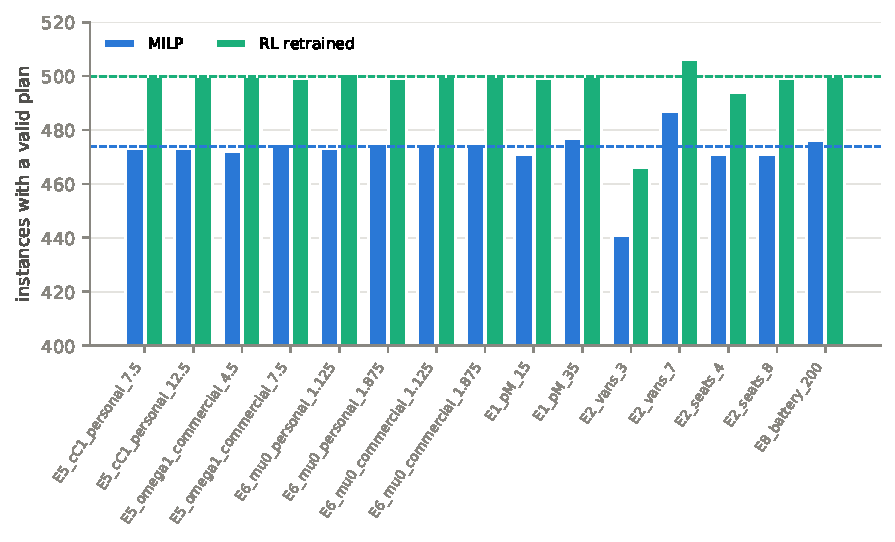
\includegraphics[width=0.95\textwidth]{figures/exp_valid.pdf}
\caption{Instances with a valid plan per variant (MILP vs RL retrained); dashed lines are the baseline.}
\label{fig:expvalid}
\end{figure}
On instances optimal in both runs the cost change from the fleet size is \textbf{0.000\,\%} (Table~\ref{tab:direction}):
the plans use only about 2.2 vans, so the fifth is rarely needed for cost. But 3 vans lose 33 instances and 7 vans
gain 13 --- almost all large R1/RC1 instances (Figure~\ref{fig:expvalid}). Cutting seats to 4 raises $Z$ about
1.1\,\% (1.3\,\% at the optima) and drops the personal van share 19.8\,\% $\to$ 11.6\,\%.

\practical{Extra vans sit idle on easy instances --- the baseline fleet already covers the demand --- so they do
not lower the bill; they earn their keep only on the hard, short-period instances where many stranded or late cars
need van trips at once. Fewer seats, by contrast, bite everywhere: the operator must send out more vans to carry
the same cars, and each dispatch is a fixed cost.}

\support{Proposition~\ref{prop:e2} predicts exactly the observed split (0.000\,\% at the optima, but
feasibility moving), and the direction check records zero cost violations. The feasibility gains/losses concentrate
in R1/RC1 as the short-period theory requires, and MILP and RL agree.}

%---------------------------------------------------------------------
\subsection{E8 --- the van battery}
\label{sec:e8}
E8 raises the van battery to 200 kWh (baseline 150).

\begin{proposition}[a slack battery has no effect]
\label{prop:e8}
Raising $B_m$ relaxes \eqref{eq:vanbatt}, so $\min Z$ is non-increasing; if the battery is slack at the optimum
(seats or time bind first), the optimum --- and $Z$ --- is unchanged.
\end{proposition}
\begin{proof}
$B_m$ is the right-hand side of \eqref{eq:vanbatt}; increasing it enlarges the feasible set, so $\min Z$ is
non-increasing. By complementary slackness, a slack constraint's multiplier is zero, so a marginal change of
$B_m$ does not move the optimum.
\end{proof}

\textbf{Result.}
\begin{table}[H]\centering
\caption{E8. Van battery 200 kWh instead of 150.}
\scriptsize
\begin{adjustbox}{max width=\linewidth}
\begin{tabular}{@{}lrrrrrrrrrrr@{}}
\toprule
method & valid & paired & new & lost & \shortstack{$\Delta Z$\\\%} & \shortstack{$\Delta$\\oper. \%} & \shortstack{$\Delta$\\cust. \%} & \shortstack{van \%\\personal} & van \% comm. & vans used & \shortstack{gap to\\MILP \%} \\
\midrule
\multicolumn{12}{@{}l}{\textbf{E8\_battery\_200}: B = 200 kWh} \\
MILP & 476 & 473 & 3 & 1 & $-$0.01 & $-$0.40 & $+$0.19 & 19.9 $\to$ 18.5 & 0.7 $\to$ 0.7 & 2.14 & -- \\
RL zero-shot & 501 & 500 & 1 & 0 & $-$0.02 & $-$0.17 & $+$0.05 & 6.7 $\to$ 6.5 & 0.9 $\to$ 0.9 & 2.19 & 0.83 \\
RL retrained & 500 & 499 & 1 & 1 & $-$0.07 & $-$0.06 & $-$0.07 & 6.7 $\to$ 8.2 & 0.9 $\to$ 0.7 & 2.18 & 0.77 \\
\bottomrule
\end{tabular}
\end{adjustbox}

\end{table}
$Z$ changes by $-0.01$\,\% on average ($-0.04$\,\% at the optima): the battery almost never binds --- seats and
time run out first. By the rule fixed before the run (an effect below 1\,\% is negligible), \textbf{van recharging
need not be modelled}.

\practical{In a one-period plan a van makes a handful of stops; its seats and the deadline cap the route long
before its battery would. So a bigger tank changes nothing the operator can use.}

\support{Proposition~\ref{prop:e8} predicts the near-zero effect from complementary slackness; the direction check
confirms a weak decrease with no violation, and both methods report essentially 0\,\%.}
